% ----------------------------------------------------
\begin{frame}
  \titlepage
\end{frame}
% ----------------------------------------------------
\note{Recordar lo visto la semana pasada: el modelo de negociación, las tres causas del fracaso (información incompleta, problemas de compromiso, bienes indivisibles). Hoy: ¿qué pasa cuando miramos \textit{dentro} del Estado? Y ¿qué papel juegan las alianzas y las organizaciones internacionales?}


% ====================================================
\section{La política doméstica y la guerra}
% ====================================================

% ----------------------------------------------------
\begin{frame}
\frametitle{¿De quién es la guerra?}
\centering

\begin{itemize}
  \item Hasta ahora: el Estado como actor \textbf{unitario}
  \item<2-> Pero las decisiones las toman \textbf{personas}
  \begin{itemize}
    \item Líderes políticos, militares, burócratas
  \end{itemize}
  \item<2-> Y los costes y beneficios de la guerra se distribuyen de forma \textbf{desigual}
  \item<3-> ¿Puede haber actores que \textit{se beneficien} de la guerra?
\end{itemize}

\end{frame}
% ----------------------------------------------------
\note{Transición clave: dejar de ver al Estado como una ``caja negra'' y mirar dentro. Ejemplos motivadores:
\begin{itemize}
  \item Argentina 1982: la junta militar invadió las Malvinas para distraer de la crisis económica y mantener el poder
  \item Guatemala 1954: EE.UU. derrocó a Árbenz para proteger los intereses de la United Fruit Company. ¿Interés nacional o interés privado?
\end{itemize}
Los costes de la guerra los pagan los soldados y los contribuyentes; los beneficios los pueden capturar políticos, empresas, militares. Esta desigualdad es central.}

% ----------------------------------------------------
\begin{frame}
\frametitle{Actores domésticos y política exterior}
\centering

\vspace{-5pt}
\begin{tikzpicture}[scale=0.8]
  % Pyramid
  \fill[accent!8] (-3, 0) -- (3, 0) -- (0, 4.5) -- cycle;
  \draw[thick, jet!40] (-3, 0) -- (3, 0) -- (0, 4.5) -- cycle;

  % Lines
  \draw[jet!20] (-2.0, 1.5) -- (2.0, 1.5);
  \draw[jet!20] (-1.0, 3.0) -- (1.0, 3.0);

  % Labels
  \node[font=\small\bfseries, jet] at (0, 3.6) {Líderes};
  \node[font=\small, jet] at (0, 2.2) {Burocracia / Militares};
  \node[font=\small, jet] at (0, 0.7) {Grupos de interés / Público};

  % Side labels
  \node[font=\tiny\itshape, asher, anchor=west] at (3.3, 3.6) {Deciden};
  \node[font=\tiny\itshape, asher, anchor=west] at (3.3, 2.2) {Asesoran e implementan};
  \node[font=\tiny\itshape, asher, anchor=west] at (3.3, 0.7) {Influyen y pagan costes};
\end{tikzpicture}

\end{frame}
% ----------------------------------------------------
\note{Pirámide de actores domésticos (basada en Figure 4.2 de FLS):
\begin{enumerate}
  \item Líderes: tienen la autoridad de decidir. Intereses propios: ideología, poder, reelección
  \item Burocracia y militares: asesoran, implementan, y tienen intereses organizacionales (presupuesto, influencia, ascensos)
  \item Grupos de interés: empresas, lobbies étnicos, opinión pública. Su influencia depende de las instituciones
\end{enumerate}
La pregunta clave: ¿qué actores importan y cómo influyen? Eso depende de las instituciones domésticas.}

% ----------------------------------------------------
\begin{frame}
\frametitle{El efecto rally y la tentación diversoria}
\centering

\begin{itemize}
  \item \textbf{Efecto rally:} la opinión pública tiende a apoyar al gobierno ante una crisis internacional
  \item<2-> El apoyo puede ser una \textit{tentación} para líderes en problemas
  \begin{itemize}
    \item Crear una crisis externa para ganar apoyo interno
  \end{itemize}
  \item<2-> ``Lo que este país necesita es una guerra corta y victoriosa''
  \begin{itemize}
    \item {\scriptsize Ministro ruso antes de la guerra ruso-japonesa (1904)}
  \end{itemize}
\end{itemize}

\end{frame}
% ----------------------------------------------------
\note{Rally effect: la aprobación del líder sube al inicio de una crisis.
\begin{itemize}
  \item Bush tras el 11-S: de 51\% a 86\% de aprobación
  \item Thatcher tras las Malvinas: de 29\% a 51\%
  \item Argentina 1982: las manifestaciones contra la junta se convirtieron en manifestaciones de apoyo tras la invasión
\end{itemize}
¿Por qué? Patriotismo, unidad nacional, la oposición calla, los medios se alinean, se puede culpar al enemigo externo.

La tentación diversoria (diversionary incentive): un líder en crisis doméstica podría provocar una crisis internacional deliberadamente. Shakespeare, en Enrique IV: ``Para evitar complots, ocupa las mentes inquietas con conflictos extranjeros.''}

% ----------------------------------------------------
\begin{frame}
\frametitle{¿Funciona la guerra diversoria?}
\centering

\begin{itemize}
  \item La evidencia empírica es \textbf{débil e inconsistente}
  \item<2-> ¿Por qué?
  \begin{itemize}
    \item Los beneficios del rally rara vez compensan \textit{todos} los costes
    \item La guerra es un \textbf{riesgo}: si sale mal, el líder cae
    \item Argentina: Galtieri acabó en prisión tras perder
  \end{itemize}
  \item<3-> La guerra es más un \textit{gambling for resurrection} que una estrategia segura
\end{itemize}

\end{frame}
% ----------------------------------------------------
\note{Los estudios muestran resultados mixtos: no hay una relación sistemática fuerte entre crisis doméstica y conflicto internacional. Razones:
\begin{enumerate}
  \item El rally tiene que ser mayor que los costes de guerra para \textit{ambos} Estados. Difícil
  \item La guerra puede salir mal: Galtieri fue a prisión, el zar cayó por la guerra ruso-japonesa, Johnson no se presentó a la reelección por Vietnam
  \item ``Gambling for resurrection'': como un equipo de hockey que saca al portero en los últimos minutos -- solo tiene sentido si ya estás perdiendo con seguridad
\end{enumerate}
En la película \textit{Wag the Dog}, el presidente fabrica una guerra \textit{falsa}. En la realidad, no puedes controlar el resultado.}


% ====================================================
\section{Militares y grupos de interés}
% ====================================================

% ----------------------------------------------------
\begin{frame}
\frametitle{El complejo militar-industrial}
\centering

\begin{itemize}
  \item \textbf{Militares:} intereses en presupuesto, prestigio, ascensos
  \item \textbf{Industria de defensa:} beneficios de la producción de armas
  \item<2-> Eisenhower (1961): advirtió sobre la influencia de esta alianza
  \item<3-> Caso extremo: Japón en los años 30
  \begin{itemize}
    \item Los militares tomaron el control de la política exterior
    \item Resultado: expansionismo y guerra con China, EE.UU., etc.
  \end{itemize}
\end{itemize}

\end{frame}
% ----------------------------------------------------
\note{El complejo militar-industrial: la idea de que militares y empresas de defensa se benefician mutuamente de una política exterior agresiva. Eisenhower lo advirtió en su discurso de despedida.

Caso de Japón: en 1931, militares japoneses provocaron un incidente con China y se apoderaron de Manchuria. En 1932, oficiales navales asesinaron al primer ministro. Los militares gradualmente tomaron el control y condujeron a Japón a una espiral de expansión.

Pero: no todos los militares son belicistas. Un estudio de las crisis de la Guerra Fría mostró que los asesores militares de EE.UU. no eran más proclives a recomendar la fuerza que los civiles. En Irak 2003, los generales eran más cautelosos que los civiles del Pentágono. Los militares también conocen el coste de la guerra.}

% ----------------------------------------------------
\begin{frame}
\frametitle{¿Cómo influyen los grupos pequeños?}
\centering

\begin{itemize}
  \item Los que se benefician de la guerra son pocos
  \item Los que pagan los costes son muchos
  \item<2-> Pero los grupos pequeños tienen \textbf{ventajas estratégicas}:
  \begin{itemize}
    \item Más fácil organizarse y coordinar
    \item Mayor incentivo individual (mucho que ganar per cápita)
    \item El gran público sufre un problema de \textbf{acción colectiva}
  \end{itemize}
  \item<2-> {\scriptsize Guatemala: United Fruit pagó 3M\$; el coste por contribuyente fue céntimos}
\end{itemize}

\end{frame}
% ----------------------------------------------------
\note{Problema de acción colectiva: los contribuyentes estadounidenses que pagaron la intervención en Guatemala tenían un coste individual de céntimos. Ninguno tiene incentivo para informarse, llamar a su congresista, etc. United Fruit, en cambio, se jugaba 16 millones de dólares.

Mecanismos de influencia:
\begin{itemize}
  \item Dinero: donaciones de campaña, el flujo de recursos entre industria y gobierno
  \item Información: los militares controlan la inteligencia que recibe el líder. Pueden sesgar los datos para favorecer la opción bélica
  \item Votos: lobbies como AIPAC o el lobby cubano-americano movilizan votantes en temas específicos
\end{itemize}
Pero ojo: los grupos de interés no siempre quieren guerra. Las empresas con comercio internacional a menudo presionan por la paz.}

% ----------------------------------------------------
\begin{frame}
\frametitle{Efecto en la negociación internacional}
\centering

\begin{itemize}
  \item Los actores domésticos belicistas no suelen \textit{causar} la guerra directamente
  \item<2-> Pero \textbf{amplían las ambiciones} del Estado:
  \begin{itemize}
    \item Más cosas por las que estarían dispuestos a luchar
    \item Demandas mayores al adversario
    \item Más oportunidades de conflicto
  \end{itemize}
  \item<2-> Para que haya guerra, siguen haciendo falta los problemas de negociación del capítulo anterior
\end{itemize}

\end{frame}
% ----------------------------------------------------
\note{Punto clave: la influencia de actores belicistas dentro del Estado no elimina el rango de negociación (excepto en casos extremos). Lo que hace es:
\begin{itemize}
  \item Reducir los costes percibidos de la guerra (para quienes deciden)
  \item Ampliar el conjunto de bienes sobre los que el Estado está dispuesto a luchar
  \item Hacer que el Estado haga demandas mayores
\end{itemize}
Esto crea más \textit{oportunidades} de conflicto, pero para que la guerra estalle, siguen necesitándose los problemas de información incompleta, compromisos no creíbles o bienes indivisibles.}

% ----------------------------------------------------
\begin{frame}
\centering
\vspace{30pt}

{\large La invasión de las Malvinas (1982): ¿fue una guerra diversoria de la junta argentina?}

\vspace{15pt}
\footnotesize ¿Qué actores domésticos influyeron y qué esperaban ganar?

\end{frame}
% ----------------------------------------------------
\note{Pregunta de discusión que conecta todo lo visto. La junta militar argentina enfrentaba protestas masivas y crisis económica. Galtieri creyó que una ``guerra corta y victoriosa'' le daría legitimidad. El efecto rally funcionó brevemente: las protestas se transformaron en apoyo. Pero la guerra se perdió, la junta cayó y Galtieri fue juzgado. Conectar con: rally effect (funcionó), gambling for resurrection (salió mal), militares tomando decisiones (sin contrapeso civil), problema de información (subestimaron la determinación británica). Un caso que ilustra todos los conceptos de esta sección.}


% ====================================================
\section{La paz democrática}
% ====================================================

% ----------------------------------------------------
\begin{frame}
\frametitle{La paz democrática}
\centering

\begin{itemize}
  \item Observación empírica: hay muy pocos (o ningún) casos claros de guerra entre \textbf{democracias maduras}
  \item<2-> Pero las democracias \textbf{sí} luchan contra no-democracias
  \item<2-> No son más pacíficas en general -- solo entre ellas
  \vspace{8pt}
  \item<3-> ¿Por qué?
\end{itemize}

\end{frame}
% ----------------------------------------------------
\note{Una de las observaciones más importantes y debatidas de las RRII. En los 200 años de democracias modernas, es difícil encontrar una guerra clara entre dos democracias consolidadas.

Casos ambiguos: la guerra de Kargil entre India y Pakistán (1999), donde ambos eran formalmente democráticos pero el ejército pakistaní manipuló al gobierno civil.

Pero las democracias no son más pacíficas en general: luchan con frecuencia contra autocracias. Hay algo específico en la relación \textit{entre} democracias.

Esto ha tenido enorme influencia política: Bush justificó la promoción de la democracia en Oriente Medio con este argumento; Obama lo citó en su discurso del Nobel.}

% ----------------------------------------------------
\begin{frame}
\frametitle{¿Por qué las democracias no luchan entre sí?}
\centering

\footnotesize
\begin{tabular}{>{\bfseries}l p{6.5cm}}
Rendición de cuentas & Los líderes democráticos pagan costes políticos más altos por guerras costosas o perdidas \\[8pt]
\onslide<2->{Transparencia & Los procesos democráticos son más abiertos: prensa libre, debate legislativo, oposición. Reduce la incertidumbre} \\[8pt]
\onslide<3->{Señales creíbles & Las amenazas de líderes democráticos son más creíbles (costes de audiencia mayores)} \\[8pt]
\onslide<4->{Normas compartidas & Las democracias se perciben como parte de una ``comunidad'' que resuelve disputas pacíficamente} \\
\end{tabular}

\end{frame}
% ----------------------------------------------------
\note{Cuatro mecanismos complementarios:
\begin{enumerate}
  \item Rendición de cuentas (accountability): las elecciones permiten castigar a líderes que hacen guerras costosas. Truman, Johnson, Bush II -- todos sufrieron políticamente por guerras impopulares. Los líderes autocráticos pueden sobrevivir a derrotas (Saddam después de 1991)
  \item Transparencia: la prensa libre, los debates parlamentarios y la oposición hacen más difícil ocultar información. Un adversario democrático puede observar mejor las capacidades y la determinación. Esto reduce la información incompleta
  \item Señales creíbles: si un presidente democrático amenaza públicamente, retirarse le costaría mucho (costes de audiencia). Por tanto, sus amenazas son más informativas
  \item Normas: las democracias se ven entre sí como legítimas y merecedoras de respeto. No aplican la misma cortesía a autocracias
\end{enumerate}}

% ----------------------------------------------------
\begin{frame}
\frametitle{¿La democracia causa la paz?}
\centering

\begin{itemize}
  \item Correlación $\neq$ causalidad
  \item<2-> Explicaciones alternativas:
  \begin{itemize}
    \item ¿El desarrollo económico causa \textit{tanto} democracia como paz?
    \item ¿Es la paz la que permite la democracia?
    \item ¿Las democracias de la Guerra Fría eran pacíficas entre sí por un enemigo común (URSS)?
  \end{itemize}
  \vspace{8pt}
  \item<3-> El debate sigue abierto
\end{itemize}

\end{frame}
% ----------------------------------------------------
\note{Tres argumentos escépticos:
\begin{enumerate}
  \item Causa común: el desarrollo económico favorece tanto la democracia como la paz (``paz capitalista'')
  \item Causalidad inversa: la democracia es más probable en entornos pacíficos. Los países con amenazas externas constantes tienden a regímenes autoritarios
  \item Variable omitida: durante la Guerra Fría, las democracias eran aliadas contra la URSS. Su paz entre ellas podría explicarse por intereses estratégicos comunes, no por sus instituciones
\end{enumerate}
Estos argumentos no refutan la paz democrática pero nos obligan a ser cautelosos. También: Hitler llegó al poder democráticamente y luego destruyó la democracia.}

% ----------------------------------------------------
\begin{frame}
\centering
\vspace{30pt}

{\large Si la democracia favorece la paz, ¿deberían los países democráticos promover la democracia en otros Estados?}

\vspace{15pt}
\footnotesize ¿Qué riesgos tendría esa política?

\end{frame}
% ----------------------------------------------------
\note{Pregunta de discusión sobre implicaciones políticas de la paz democrática. Bush usó este argumento para justificar la invasión de Irak y la ``agenda de libertad'' en Oriente Medio. Riesgos: las transiciones democráticas son inestables y pueden aumentar temporalmente el riesgo de guerra (Mansfield y Snyder); la imposición externa puede generar rechazo nacionalista; puede ser un pretexto para intervención imperialista. Conectar con la idea de que la correlación no implica causalidad: forzar la democracia no es lo mismo que la democratización orgánica.}


% ====================================================
\section{Alianzas}
% ====================================================

% ----------------------------------------------------
% IMAGE: nato_warsaw_map -- Mapa de Europa mostrando los bloques OTAN vs Pacto de Varsovia durante la Guerra Fría
% TODO: uncomment when image is available
% \begin{frame}[plain]
%   \begin{tikzpicture}[remember picture, overlay]
%     \node[at = (current page.center), yshift = 0cm] (cover) {%
%       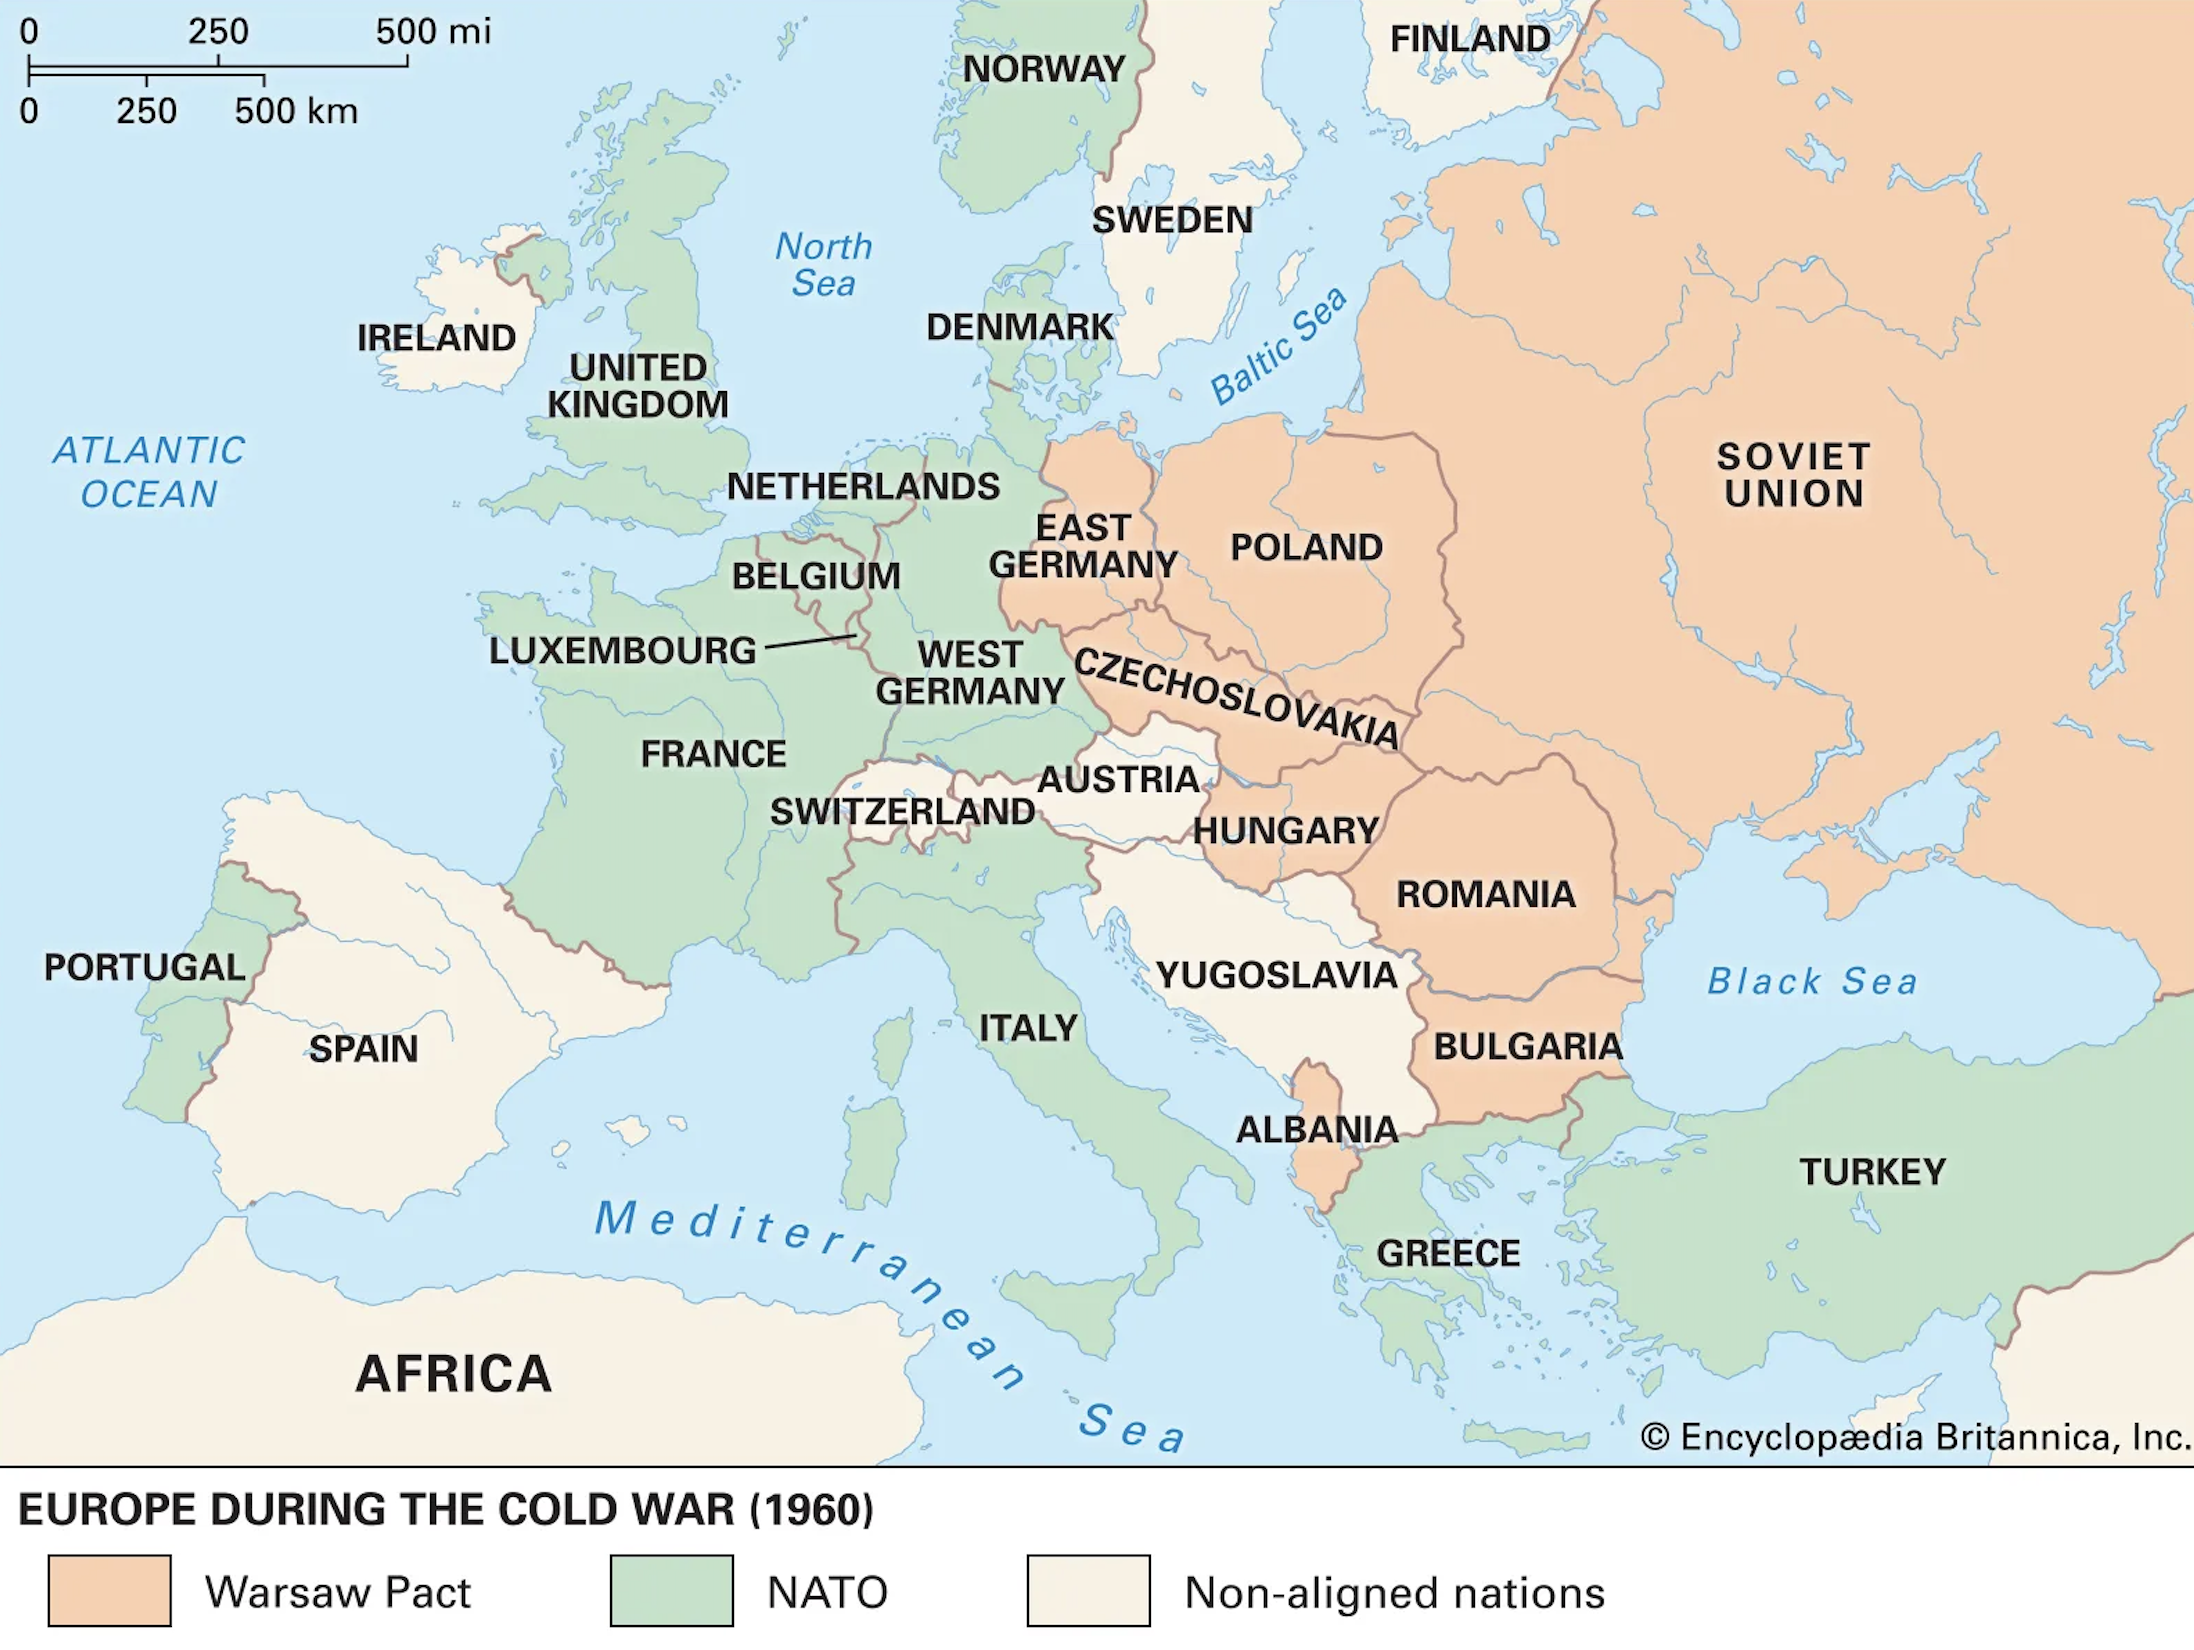
\includegraphics[keepaspectratio, height=\paperheight]{../img/nato_warsaw_map}};
%   \end{tikzpicture}
% \end{frame}
% % ----------------------------------------------------
% \note{Mapa de los dos bloques durante la Guerra Fría: OTAN (azul) vs. Pacto de Varsovia (rojo). Visualiza la bipolaridad del sistema internacional. La línea divisoria cruzaba Europa, con Alemania dividida en dos. Las alianzas definieron las interacciones entre Estados durante casi medio siglo.}

% ----------------------------------------------------
\begin{frame}
\frametitle{Alianzas}
\centering

\begin{itemize}
  \item Acuerdos de cooperación militar entre Estados
  \item<2-> \textbf{Defensivas:} ``si te atacan, te defiendo''
  \item<2-> \textbf{Ofensivas:} ``atacamos juntos'' (menos comunes)
  \item<3-> Función principal: señalar intereses comunes e influir en el comportamiento de \textbf{terceros}
\end{itemize}

\end{frame}
% ----------------------------------------------------
\note{Las alianzas son instituciones que buscan hacer creíble la promesa de ayuda mutua. La más importante: la OTAN (1949). EE.UU. también tiene alianzas bilaterales con Japón, Corea del Sur, Filipinas y Australia.

Las alianzas son un mecanismo de disuasión extendida: ``no ataques a mi aliado o te enfrentarás a los dos''. Esto cambia el cálculo del adversario potencial: ahora tiene que considerar la intervención de un tercero.

Las alianzas influyen en el modelo de negociación al cambiar las expectativas sobre lo que pasará en caso de guerra (el resultado esperado).}

% ----------------------------------------------------
\begin{frame}
\frametitle{El dilema de las alianzas}
\centering

\begin{itemize}
  \item \textbf{Abandono:} ¿y si mi aliado no cumple cuando lo necesite?
  \begin{itemize}
    \item Si la promesa no es creíble, la disuasión falla
  \end{itemize}
  \item<2-> \textbf{Trampa} (\textit{entrapment}): ¿y si mi aliado me arrastra a una guerra que no quiero?
  \begin{itemize}
    \item Si la promesa es demasiado firme, el aliado toma más riesgos
  \end{itemize}
  \item<3-> Trade-off entre credibilidad y control
\end{itemize}

\end{frame}
% ----------------------------------------------------
\note{Dilema fundamental de las alianzas:
\begin{itemize}
  \item Abandonamiento: si EE.UU. deja de proteger a Taiwán, China puede atacar. Si la OTAN no responde a un ataque contra Estonia, pierde toda credibilidad
  \item Entrapment: si la alianza es demasiado firme, el aliado puede asumir riesgos que de otra forma no tomaría. Ejemplo: el ``cheque en blanco'' de Alemania a Austria-Hungría en 1914 animó a Austria a ser más agresiva con Serbia
\end{itemize}
Cómo se gestiona: compromisos específicos (``te defiendo contra X, pero no contra Y''), mantener cierta ambigüedad estratégica (EE.UU. con Taiwán).

Evidencia: las alianzas generalmente funcionan para disuadir ataques contra sus miembros.}

% ----------------------------------------------------
\begin{frame}
\frametitle{El equilibrio de poder y la Guerra Fría}
\centering

\begin{itemize}
  \item La OTAN y el Pacto de Varsovia dividieron el mundo en dos
  \item<2-> \textbf{Bipolaridad:} dos bloques claros, menos incertidumbre
  \begin{itemize}
    \item Cada Estado sabía quién estaba con quién
  \end{itemize}
  \item<2-> Resultado: ninguna guerra directa entre las superpotencias
  \item<3-> ¿Pero a qué coste? Guerras proxy en el ``Tercer Mundo''
\end{itemize}

\end{frame}
% ----------------------------------------------------
\note{La estructura bipolar de la Guerra Fría puede haber contribuido a la ``larga paz'' entre grandes potencias (1953-presente). La bipolaridad reduce la incertidumbre: cada bando sabe quién se le va a enfrentar. Contraste con la multipolaridad de 1914 (más actores, más incertidumbre).

Pero la paz entre superpotencias vino acompañada de guerras proxy devastadoras: Corea, Vietnam, Afganistán, Angola, Centroamérica. Las superpotencias luchaban a través de aliados y rebeldes locales.

Alternativa al equilibrio: \textit{bandwagoning} -- aliarse con el más fuerte para compartir las ganancias, en vez de equilibrar al más fuerte. Menos común pero existe.}


% ====================================================
\section{Seguridad colectiva}
% ====================================================

% ----------------------------------------------------
\begin{frame}
\frametitle{Seguridad colectiva}
\centering

\begin{itemize}
  \item A diferencia de las alianzas (selectivas), la seguridad colectiva aspira a incluir a \textbf{todos} los Estados
  \item<2-> Principio: un ataque contra uno es un ataque contra todos
  \begin{itemize}
    \item Sociedad de Naciones (1919), ONU (1945)
  \end{itemize}
  \item<3-> Objetivo: disuadir la agresión haciendo que el coste sea enfrentarse al mundo entero
\end{itemize}

\end{frame}
% ----------------------------------------------------
\note{La seguridad colectiva es una idea ambiciosa: si todos los Estados prometen defender a cualquier Estado que sea atacado, nadie se atreverá a atacar. Es la lógica detrás de la Sociedad de Naciones (fracasó) y la ONU.

Diferencia con alianzas: las alianzas son selectivas (OTAN no incluye a Rusia); la seguridad colectiva aspira a ser universal. Incluye la idea de que los cambios al statu quo deben ser pacíficos.

El concepto se ha expandido: originalmente solo cubría agresión interestatal. Desde el fin de la Guerra Fría, incluye intervención en guerras civiles, genocidio, violaciones masivas de DDHH (``responsabilidad de proteger'').}

% ----------------------------------------------------
\begin{frame}
\frametitle{El problema de la acción colectiva}
\centering

\begin{itemize}
  \item La seguridad colectiva es un \textbf{bien público}
  \item<2-> Problema del \textit{free rider}:
  \begin{itemize}
    \item Todos se benefician de la paz, pero nadie quiere pagar el coste de mantenerla
    \item Sanciones, tropas, cascos azules -- todo es costoso políticamente
  \end{itemize}
  \item<3-> Solución imperfecta: concentrar la decisión en pocos actores
  \begin{itemize}
    \item El Consejo de Seguridad de la ONU
  \end{itemize}
\end{itemize}

\end{frame}
% ----------------------------------------------------
\note{El mismo dilema del prisionero que vimos en la sesión 2, aplicado a la seguridad internacional. Enviar tropas para mantener la paz en un país lejano es costoso y políticamente impopular. Cada Estado prefiere que otros lo hagan.

La ONU intenta resolver esto concentrando la decisión en el Consejo de Seguridad:
\begin{itemize}
  \item 15 miembros, 5 permanentes con veto (EE.UU., Rusia, China, Francia, UK)
  \item Si los P5 están de acuerdo, la acción tiene respaldo de las principales potencias
  \item Pero si están en desacuerdo (como en Siria), el Consejo se paraliza
\end{itemize}
Solo dos casos de respuesta militar colectiva a gran escala a una agresión: Corea (1950) y Kuwait (1991). Ambos fueron posibles por circunstancias excepcionales.}

% ----------------------------------------------------
\begin{frame}
\frametitle{Operaciones de paz de la ONU}
\centering

\begin{itemize}
  \item \textbf{Peacekeeping} (mantenimiento de paz):
  \begin{itemize}
    \item Cascos azules, ligeramente armados
    \item Separar a los combatientes tras un alto el fuego
    \item Requiere consentimiento de las partes
  \end{itemize}
  \item<2-> \textbf{Peace enforcement} (imposición de paz):
  \begin{itemize}
    \item Mayor uso de la fuerza autorizado
    \item State-building: elecciones, instituciones
    \item No requiere consentimiento
  \end{itemize}
\end{itemize}

\end{frame}
% ----------------------------------------------------
\note{Dos tipos de operaciones:
\begin{enumerate}
  \item Peacekeeping (cascos azules): tropas bajo mando de la ONU que ocupan una zona de separación. Evitan el combate y construyen confianza. Funcionan bien cuando las partes quieren la paz. Limitaciones serias: Ruanda (1994) -- los cascos azules estaban presentes pero no tenían mandato para intervenir. Srebrenica (1995) -- cascos azules holandeses no pudieron impedir la masacre
  \item Peace enforcement: intervenciones más robustas. Ejemplo: la OTAN en Kosovo (1999), la intervención en Libia (2011). Incluyen a menudo actividades de state-building (elecciones, reconstrucción institucional)
\end{enumerate}
Explosión de operaciones de paz desde 1990: de unas pocas a decenas. Pero siguen siendo limitadas por la voluntad política de los miembros.}

% ----------------------------------------------------
\begin{frame}
\frametitle{Las organizaciones internacionales y la negociación}
\centering

\begin{itemize}
  \item Tres formas en que las OO.II. influyen:
  \begin{enumerate}
    \item<2-> Hacen la guerra \textbf{menos atractiva} (amenaza de intervención)
    \item<3-> Ayudan a resolver \textbf{problemas de compromiso} (monitoreo, verificación)
    \item<4-> Sirven como \textbf{observadores neutrales} y mediadores
  \end{enumerate}
\end{itemize}

\end{frame}
% ----------------------------------------------------
\note{Conectar con el modelo de negociación del capítulo 3:
\begin{enumerate}
  \item La posibilidad de que la comunidad internacional intervenga aumenta los costes esperados de iniciar una guerra. Amplía el rango de negociación
  \item Los peacekeepers pueden garantizar que se cumplen los acuerdos. Si ambas partes confían en que la ONU verificará el desarme, es más fácil llegar a un acuerdo (resuelve problemas de compromiso)
  \item Los observadores neutrales reducen la incertidumbre: la OIEA verifica programas nucleares; los observadores electorales confirman resultados
\end{enumerate}
Pero la ONU es imperfecta: depende de la voluntad de sus miembros, sobre todo de los P5. Soberanía y competencia entre grandes potencias limitan su efectividad.}


% ====================================================

% ----------------------------------------------------
\begin{frame}
\frametitle{Resumen (marco I-I-I)}
\centering

\begin{itemize}
  \item \textbf{Intereses:} líderes, militares y grupos de interés tienen intereses propios que pueden ampliar las ambiciones del Estado
  \item<2-> \textbf{Interacciones:} la democracia cambia cómo interactúan los Estados (transparencia, señales creíbles, rendición de cuentas) $\rightarrow$ paz democrática
  \item<3-> \textbf{Instituciones:} alianzas, seguridad colectiva y OO.II. influyen en la negociación cambiando expectativas, credibilidad y costes
\end{itemize}

\end{frame}
% ----------------------------------------------------
\note{Resumen de los dos ejes de esta sesión:
\begin{enumerate}
  \item La política doméstica importa: quién gobierna y a quién rinde cuentas afecta a la probabilidad de guerra. Pero los actores belicistas domésticos rara vez causan la guerra por sí solos
  \item La democracia reduce la guerra entre democracias, pero no la guerra en general
  \item Las alianzas y la seguridad colectiva son instituciones que influyen en el modelo de negociación, pero tienen problemas propios (abandono, trampa, free riding, veto en el Consejo de Seguridad)
\end{enumerate}
La próxima semana: violencia por actores no estatales -- guerras civiles y terrorismo.}

% ----------------------------------------------------
\begin{frame}
\frametitle{}
\centering

Preguntas?

\end{frame}
% ----------------------------------------------------
\note{}
